\documentclass[10pt, xcolor=dvipsnames]{beamer}

\usetheme{metropolis}
\usepackage[utf8]{inputenc}
\usepackage[english]{babel}
\usepackage{ragged2e}
\usepackage{bbding}
%\usepackage{enumitem}
\usepackage{mathtools}
\usepackage{indentfirst}
\usepackage{graphicx}
\usepackage{float}
\usepackage{hyperref}
\usepackage{mathtools}
\usepackage{preview}
\usepackage{xcolor}
\usepackage{color}
\usepackage{listings}
\usepackage{float}
\usepackage[caption = false]{subfig}
\usepackage{pdfpages}
\usepackage{multirow}
\usepackage{array}
\usepackage{makecell}
\usepackage{bm}
\usepackage{caption}
\usepackage{cancel}
\usepackage{anyfontsize}
\usepackage{etoolbox}
\usepackage{amsmath}
\usepackage{amssymb}
\usepackage{mathtools}
\usepackage{natbib}
\usepackage[flushleft]{threeparttable}
\usepackage{booktabs}
\usepackage{caption}
\usepackage{adjustbox}
\usepackage{appendixnumberbeamer}
\usepackage{pifont}
\usepackage{amsmath}
\usepackage{amssymb}
\usepackage[percent]{overpic}



\setbeamercolor{titlelike}{parent=structure}
\definecolor{UBCblue}{rgb}{0.04706, 0.13725, 0.32}
\colorlet{UBCblue2}{UBCblue!70!white}
\usecolortheme[named=UBCblue]{structure}

\makeatletter
\setbeamertemplate{footline}
{
  \leavevmode%
  \hbox{%
  \begin{beamercolorbox}[wd=.4\paperwidth,ht=2.25ex,dp=1ex,center]{author in head/foot}%
    \usebeamerfont{author in head/foot} \insertshortauthor %\hspace*{1em}(\insertshortinstitute)
  \end{beamercolorbox}%
  \begin{beamercolorbox}[wd=.5\paperwidth,ht=2.25ex,dp=1ex,center]{title in head/foot}%
    \usebeamerfont{title in head/foot} \insertshorttitle
  \end{beamercolorbox}%
  \begin{beamercolorbox}[wd=.1\paperwidth,ht=2.25ex,dp=1ex,center]{date in head/foot}%
    \usebeamerfont{date in head/foot}
    \insertframenumber{} / \inserttotalframenumber\hspace*{2ex} 
  \end{beamercolorbox}}%
  \vskip0pt%
}
\makeatother

\renewcommand{\arraystretch}{1.2}
\renewcommand{\raggedright}{\leftskip=0pt \rightskip=0pt plus 0cm}
\newcolumntype{C}[1]{>{\centering\let\newline\\\arraybackslash\hspace{0pt}}m{#1}}

\hypersetup{
    colorlinks=true,
    linkcolor=UBCblue,
    citecolor=UBCblue,
    filecolor=magenta,      
    urlcolor=blue,
    allcolors=.
}
\setbeamercolor{button}{bg=UBCblue2,fg=white}
\newcommand\fnote[1]{\captionsetup{font=tiny}\caption*{#1}}
\newcommand\fnotev[1]{\captionsetup{font=scriptsize}\caption*{#1}}
\setbeamertemplate{caption}[numbered]


%\justifying
\urlstyle{same}
%\usefonttheme{serif}

%------------------------
%------------------------

\date{}

%------------------------
%------------------------
%----------------------------------------------------------------------------------------
%	TITLE PAGE
%----------------------------------------------------------------------------------------------------------------
%------------------------

\title[How Should We Think About Low Income Rental Markets]{How Should We Think About Low Income Rental Markets} % The short title appears at the bottom of every slide, the full title is only on the title page
\author[Joe Fish]{Joe Fish}


\begin{document}

\begin{frame}
\titlepage % Print the title page as the first slide
\end{frame}

\begin{frame}{Some Facts About Low Income Rental Markets}
\textbf{Eviction}
    \begin{itemize}
        \item Eviction is common: (~8-25 evictions / 100 renter households / year)
        \begin{itemize}
            \item within high evicting neighborhoods, certain buildings will be even more high evicting
        \end{itemize}
        \item Tenant default is common and does not immediately lead to eviction
        \begin{itemize}
            \item Most eviction cases are for nonpayment of rent and for about two months of back rent
        \end{itemize}
    \end{itemize}
    \pause
\textbf{Prices and Profits}
\begin{itemize}
        \item Low Income landlords have \textbf{higher} profit margins than any other kind of landlord
        \item Rent Prices are often as high as they are in much higher quality neighborhoods; maintenance is much lower 
        \item market power due to concentration, search frictions and lack of entry likely pervasive
\end{itemize}
    
\end{frame}

\begin{frame}{Motivation}

\begin{itemize}
    \item Most US cities have awful tenant protections
    \item Tenants perceived as risky face large barriers to finding housing. Lots of rental listings will have "no eviction, no conviction" clauses, effectively locking them out of large parts of the rental market. This is true for private and public landlords.
    \item Landlords that rent to risky tenants are providing a service; these landlords are also much more likely to be predatory.
    \item When advocacy groups push for stronger tenant protections, landlords (public and private) argue that increased tenant protections would make them unable to be effective landlords. Thus, it's ex ante, unclear what the best way to regulate low income landlords is.
\end{itemize}
\end{frame}


\begin{frame}{Research questions}

\textbf{Big Picture:} \\
\vspace{0.5cm}
Are slumlords just predatory, or are they providing "housing of last resort" by renting to tenants who would otherwise be screened out by the rest of the market (or a little bit of both) \\
\vspace{0.5cm}
Are the tenants ending up in these properties just unlucky victims or are they getting access to housing they might otherwise not

\end{frame}

\begin{frame}{A Simple Model of Passive Slumlords (ASMoPS}
\textbf{Model Setup}
Landlords are passive agents who are trying to learn about tenant's ability to pay rent after an income shock; eviction does nothing except force tenant to leave after nonpayment
    \begin{itemize}
        \item step 0: landlords match with tenants; sign contract for X months
        \item tenants draw $\epsilon$ (default) from CDFs of income shocks from a known distribution
        \item based on draws, tenant does / doesn't default
        \item landlord decides whether to evict based on whether they think the tenant is likely to repay in the future
    \end{itemize}
\end{frame}

\begin{frame}{Model Implications}
Under \textbf{ASMoPS}, policies that reduce evictions can be welfare improving, but in practice they won't be.\\
\vspace{0.25cm}
Intuition: 
    \begin{itemize}
        \item Most policies that raise costs of eviction don't lead to many fewer evictions because they don't change underlying dynamics (income shocks are very common for low income tenants)
        \item Some evidence landlords pass on cost of evictions to tenants
        \item Net effect is anti-eviction policies are not super effective and may backfire
    \end{itemize}
\end{frame}

\begin{frame}{Summing Up the Passive Slumlord Model}
\begin{itemize}
    \item High rent prices explained as function of default premia 
    \item High eviction rates explained as function of renting to risky tenants
    \item Tenants are essentially \textbf{only} helped via cash transfers; regulation is likely to be \textbf{welfare negative}
\end{itemize}
    
\end{frame}

\begin{frame}{Reasons Why the Model is Wrong}
    Model predictions are very inconsistent with observed effect of reforms and explaining sustained higher \textbf{profit levels}
    \begin{figure}
    \centering
    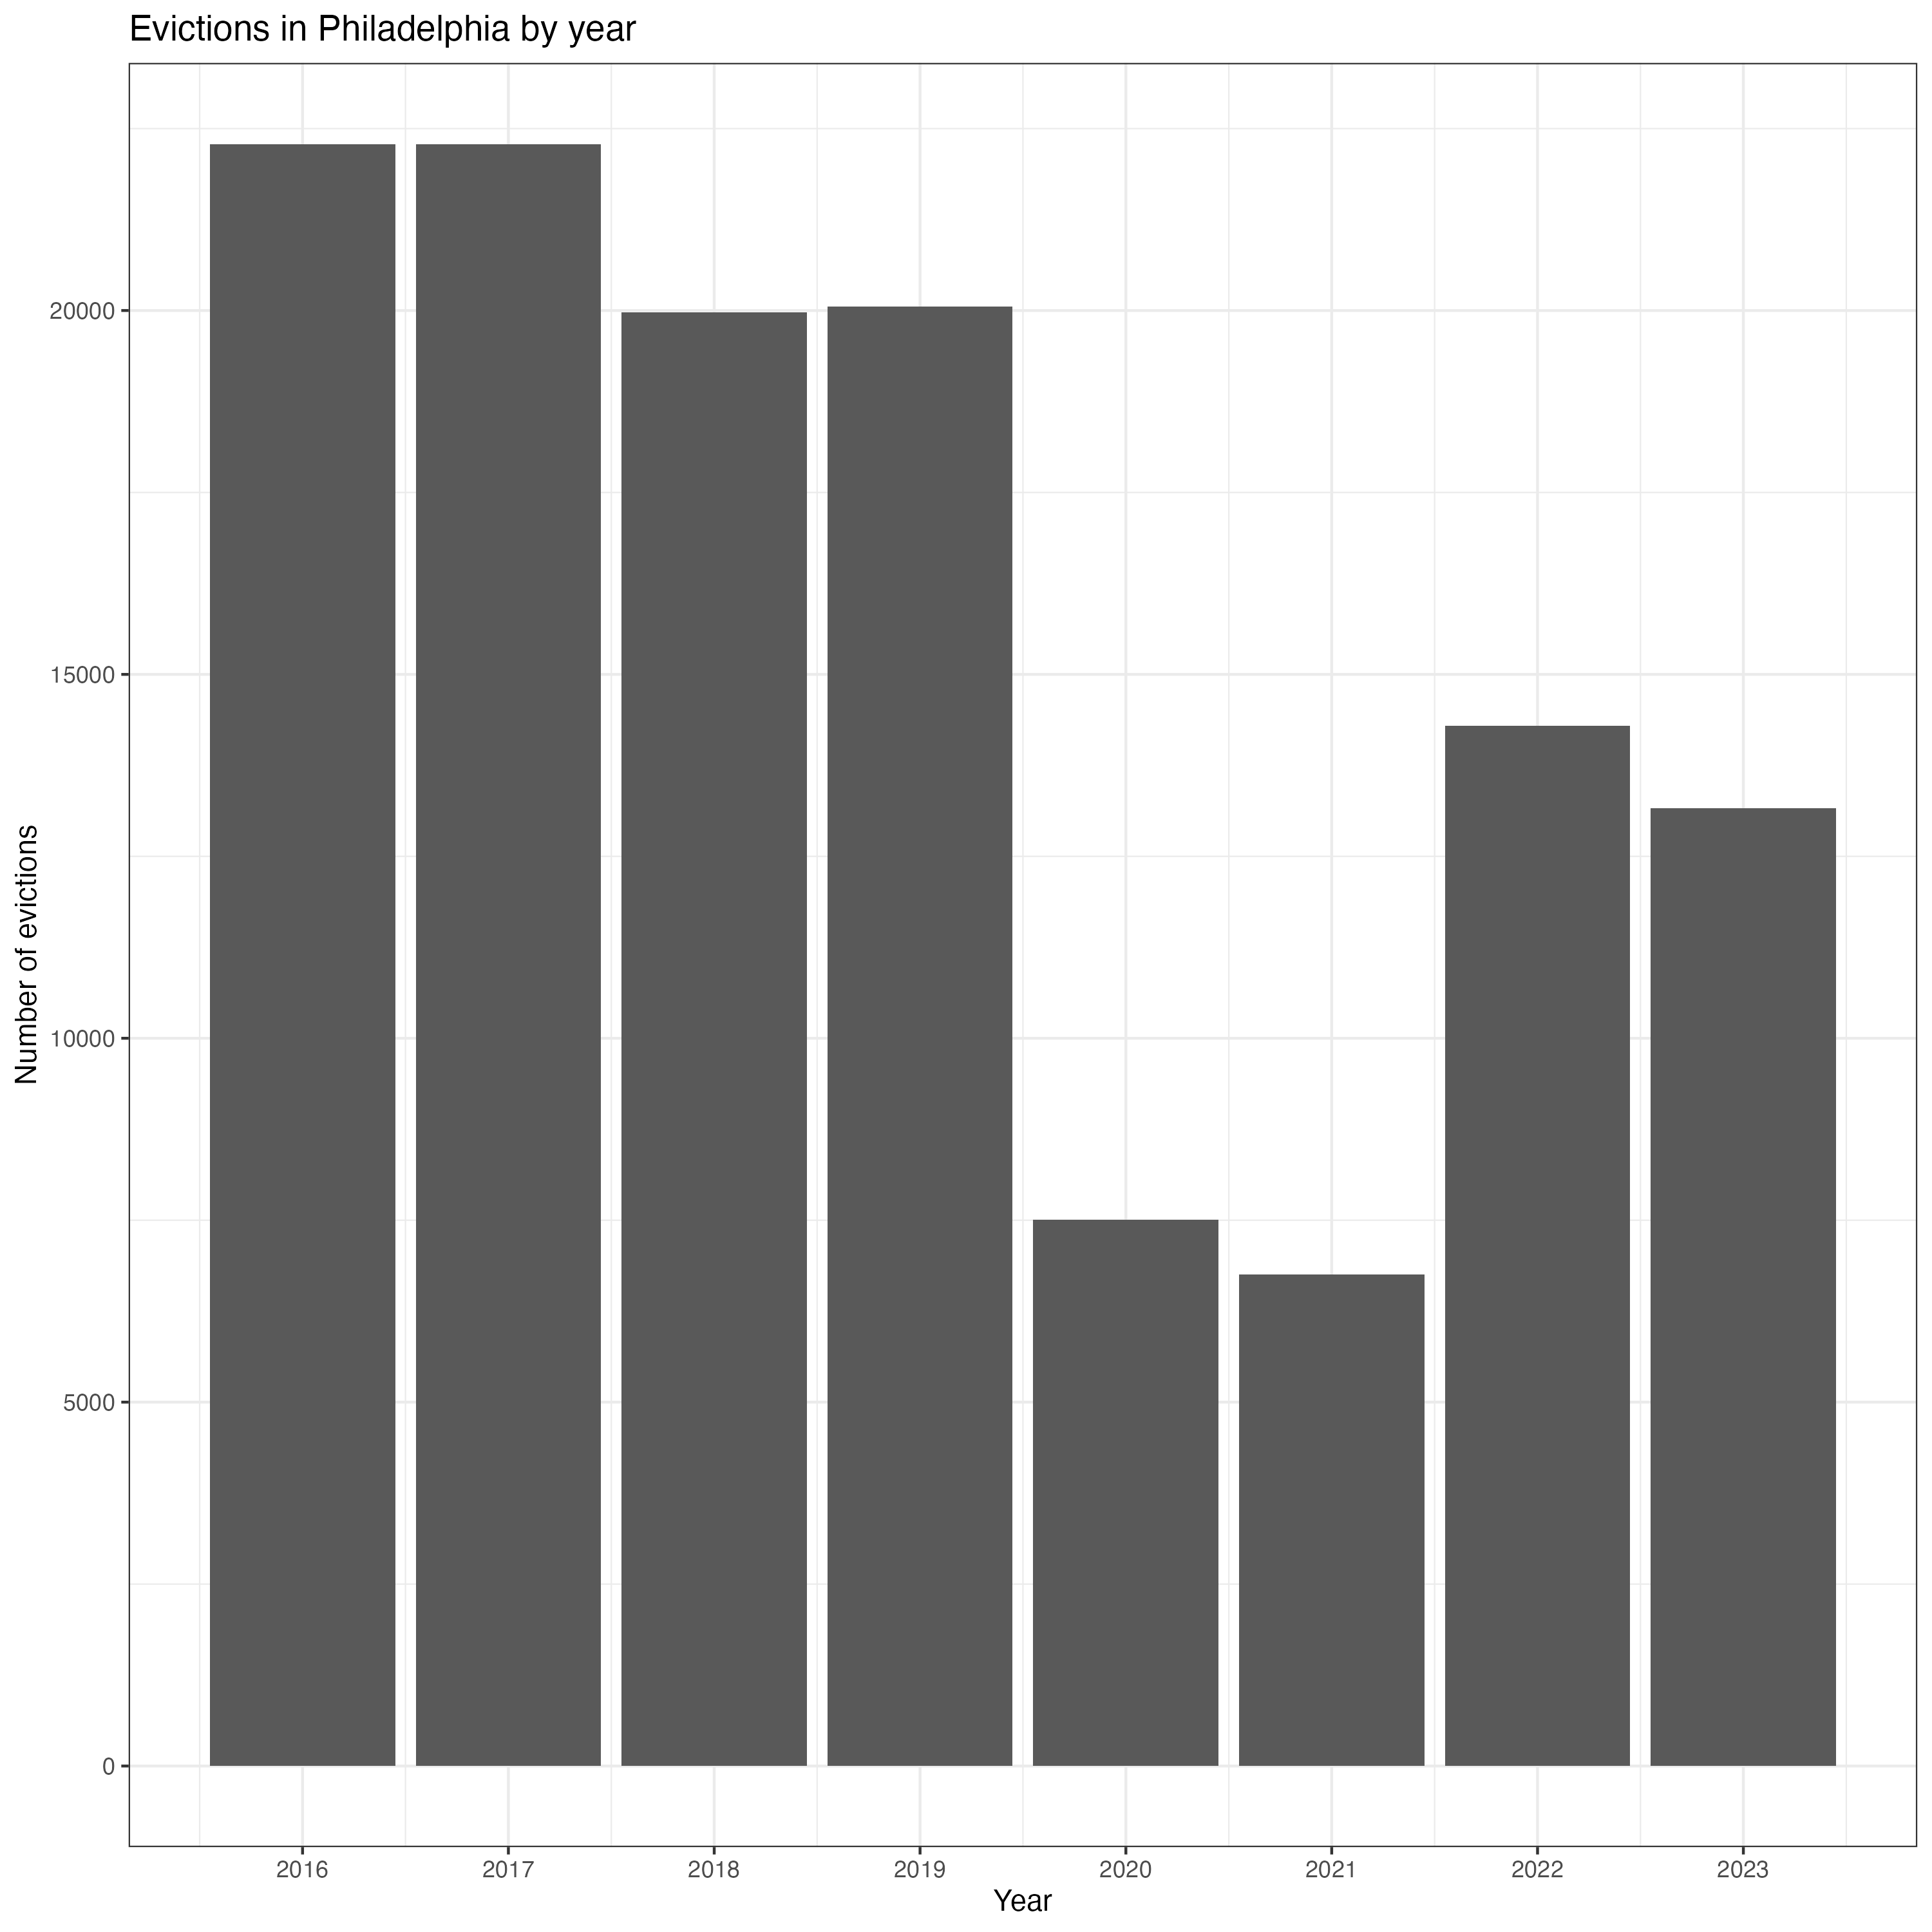
\includegraphics[width=0.5\linewidth]{figs/evict_by_year.png}
    \caption{Evictions in Philadelphia by Year}
    \label{fig:philly-ts}
\end{figure}
\end{frame}

\begin{frame}{Reasons Why the Model is Wrong}
    More broadly, low-income landlords aren't passive agents that exist only to learn about tenants' ability to repay in the future.\\
\end{frame}

\begin{frame}{A slightly more complicated model of evictions (ASMCMoE)}
Key Intuition: Threat of Eviction Serves to Prevent Tenants from Complaining
\begin{itemize}
    \item step 0: landlords match with tenants; sign contract for X months
    \item tenants and landlords draw $\epsilon$ and $\delta$ (default and something breaks) from CDFs
    \item based on draws, tenant does / doesn't default and thing does / doesn't break
    \item landlord decides whether to evict; tenant decides whether to complain
    \item if tenant decides to complain, next time tenant is in default, they are immediately evicted
\end{itemize}
\end{frame}

\begin{frame}{Problems with ASMCMoE}
    \begin{itemize}
        \item Writing and solving the model
        \item No idea if this model will actually deliver anything useful / interesting other than it might mean high evicting landlords do more maintenance
        \item Not really sure how to check whether this model is more / less true than the very simple version (can't see complaints or arrears, only building permits and evictions; complaints might be off path)
    \end{itemize}
    
\end{frame}

\begin{frame}{Pause for thoughts and questions}
    
\end{frame}

\begin{frame}{Market Power via Search Costs}
    Standard models of market power in housing have landlords flex market power by either \\
    \begin{itemize}
        \item internalizing market power during \textbf{development}
        \item restricting quantity via higher vacancy rates
    \end{itemize} 
    \pause
    \vspace{0.25cm}
    My model: Landlords flex market power in submarkets where tenants face high search costs by either:
    \begin{itemize}
        \item exploiting switching costs 
        \item capturing tenant landlord-match surplus by removing themselves from tenant's outside option
    \end{itemize}
    \vspace{0.25cm}
    Rip off David Berger's monopsony model but for housing. Feels like someone should have done this already?
\end{frame}





% \begin{frame}{Desired Feedback}
% \begin{itemize}
%     \item Framing and research question
%     \item IO Side: what are the possible responses of the low income landlords
%     \item How to do the empirics
%     \item How to model selection into high eviction homes
% \end{itemize}
    
% \end{frame}

% \begin{frame}{Philly post-COVID}
% Post COVID, Philadelphia has seen one of the largest reductions in evictions in the country. \\
% \vspace{0.5cm}
% To some extent, this can be attributed to their eviction diversion program, which made it harder to evict tenants. \\
% \vspace{0.5cm}
% Given that Philly is a poor city with a substantial Black population that experienced a large change in tenant protections, it's the ideal place to look for changes in landlord behavior. \\
% \vspace{0.5cm}
% Other benefits: Rental registry, evictions have contract rent (means I can see low income rent prices), good historical data.
    
% \end{frame}

% \begin{frame}{Evictions in Philly: Time Series}
%     \begin{figure}
%     \centering
%     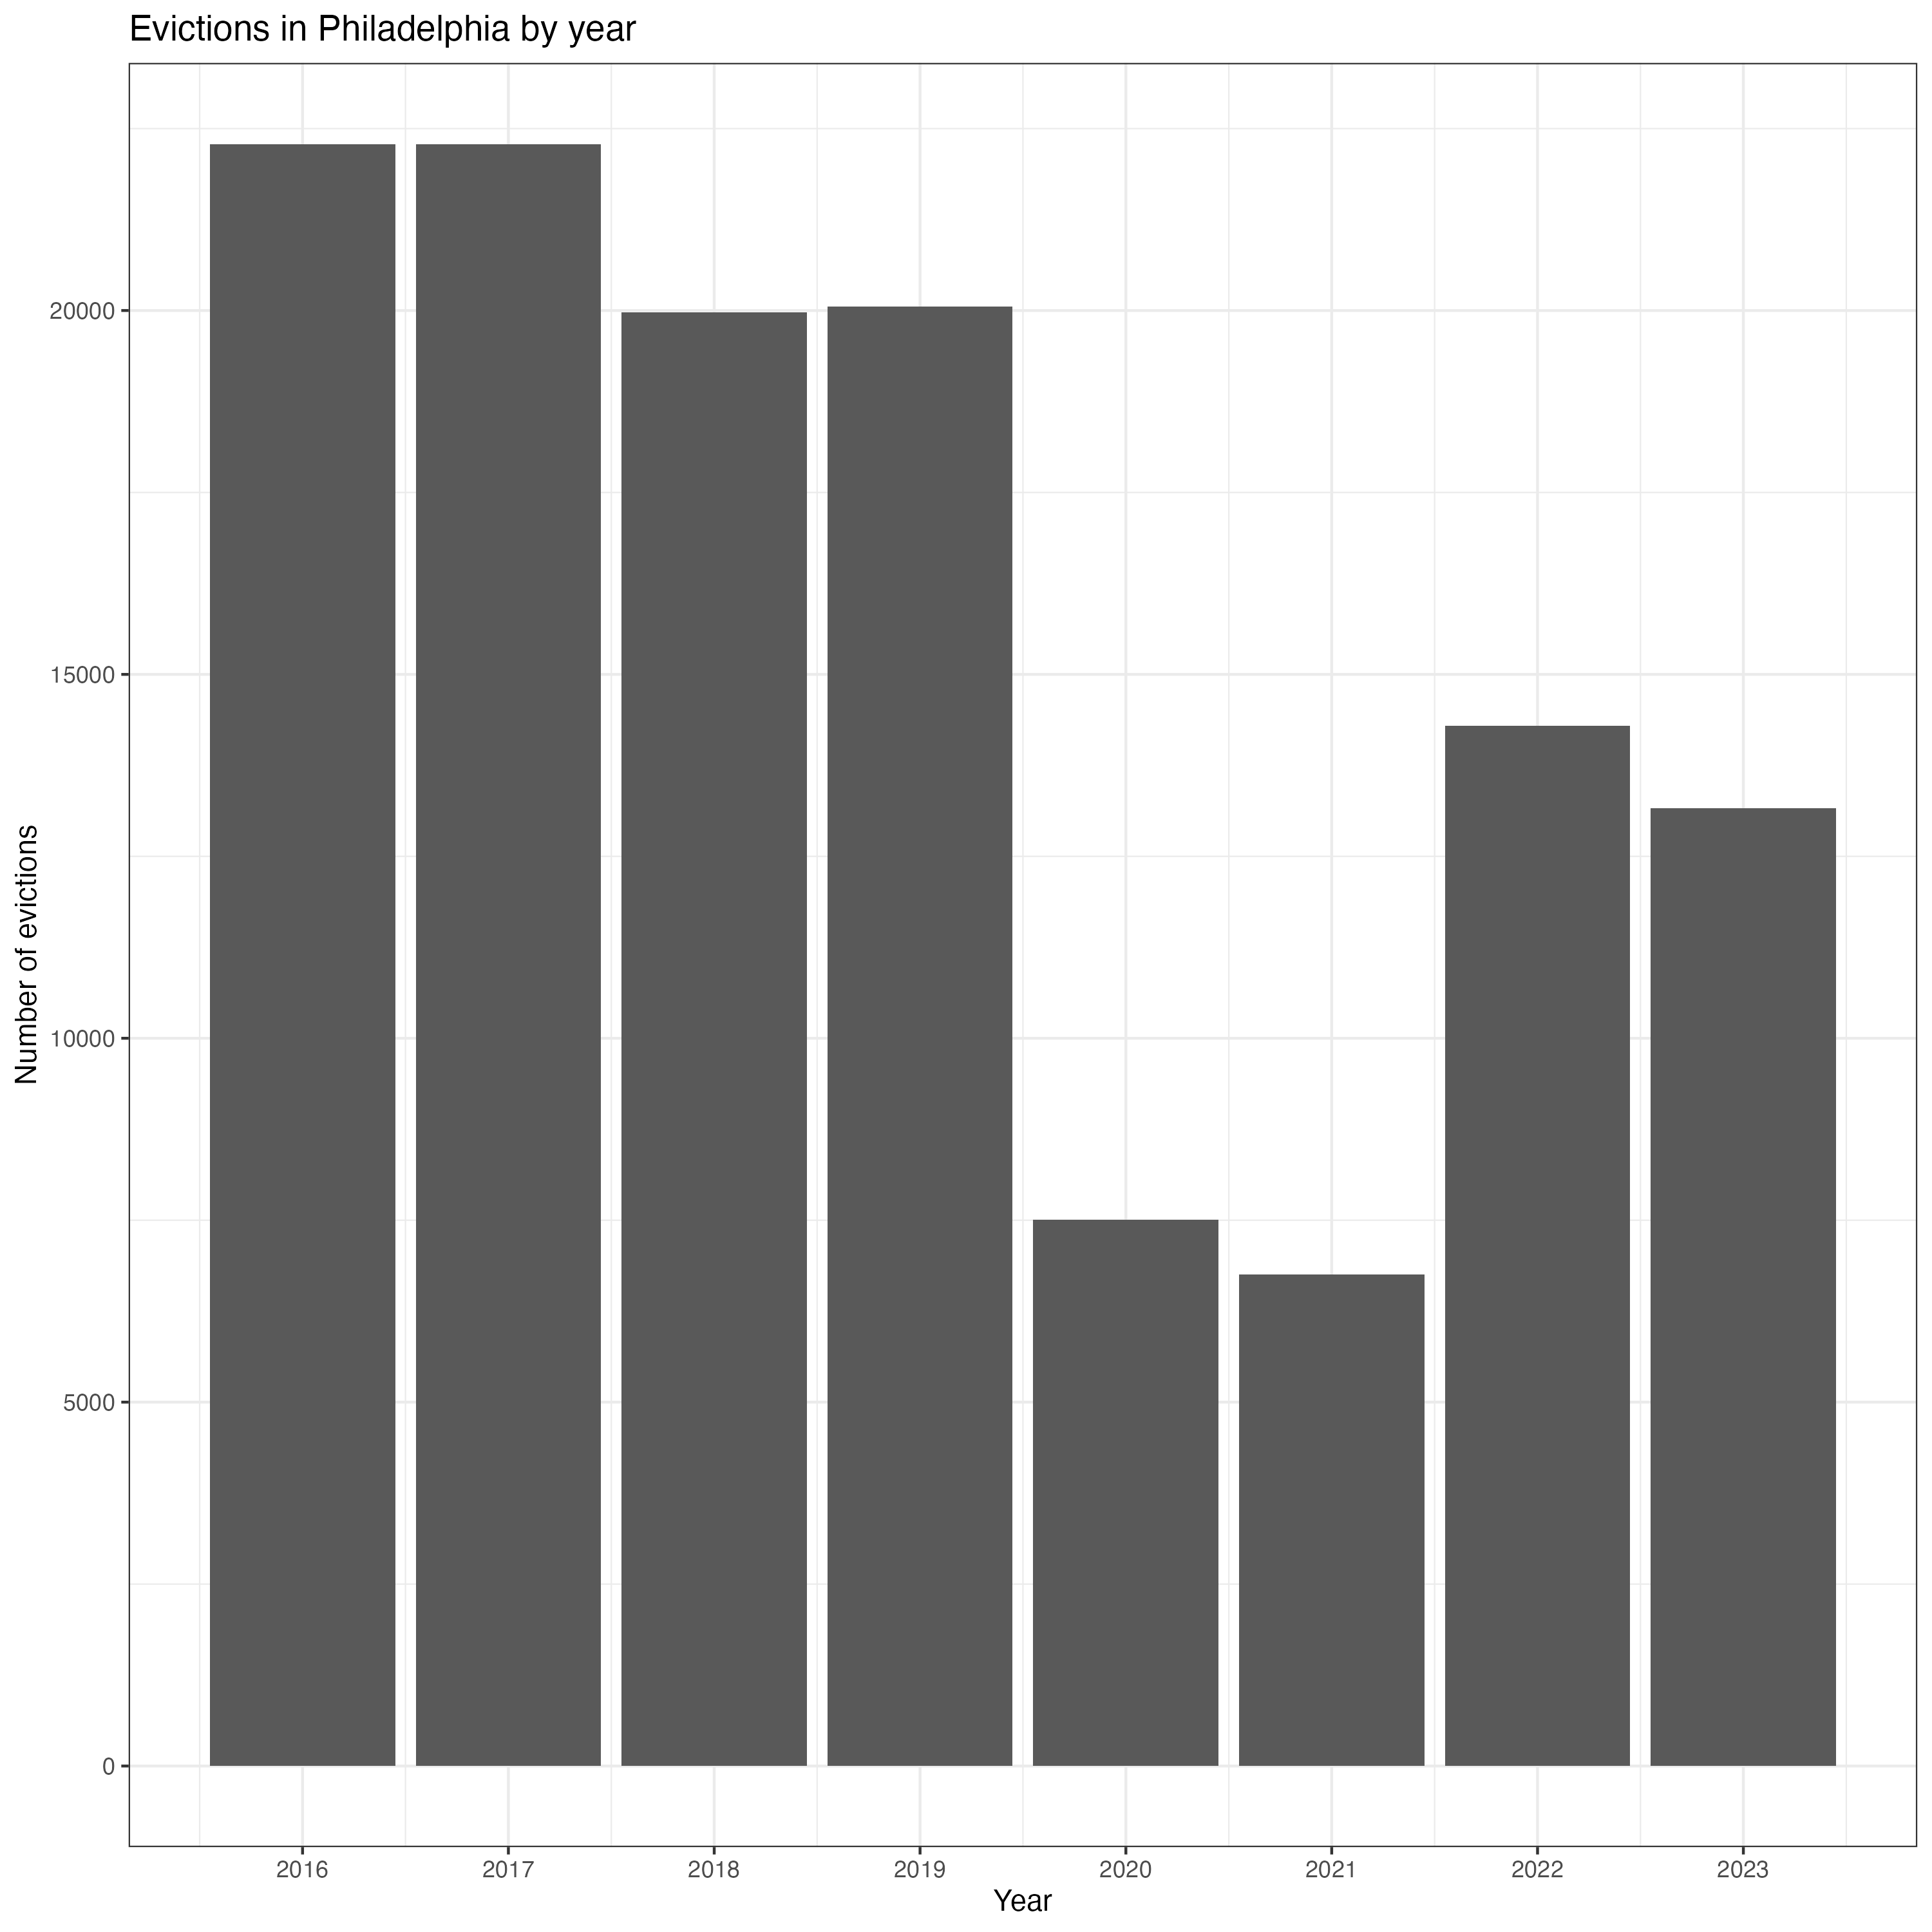
\includegraphics[width=0.5\linewidth]{figs/evict_by_year.png}
%     \caption{Evictions in Philadelphia by Year}
%     \label{fig:philly-ts}
% \end{figure}
% \end{frame}


% \begin{frame}{Evictions in America}
% \textbf{Evictions in America are heavily concentrated:}
% \begin{itemize}
%     \item They are concentrated within certain cities (poorer, Blacker ones)
%     \item Within cities, they are concentrated within certain neighborhoods (poorer, Blacker ones)
%     \item Within neighborhoods, they are concentrated within certain buildings and within specific landlords 
% \end{itemize} 

    
% \end{frame}

% \begin{frame}{Evictions in America: National}
% \begin{figure}
%     \centering
%     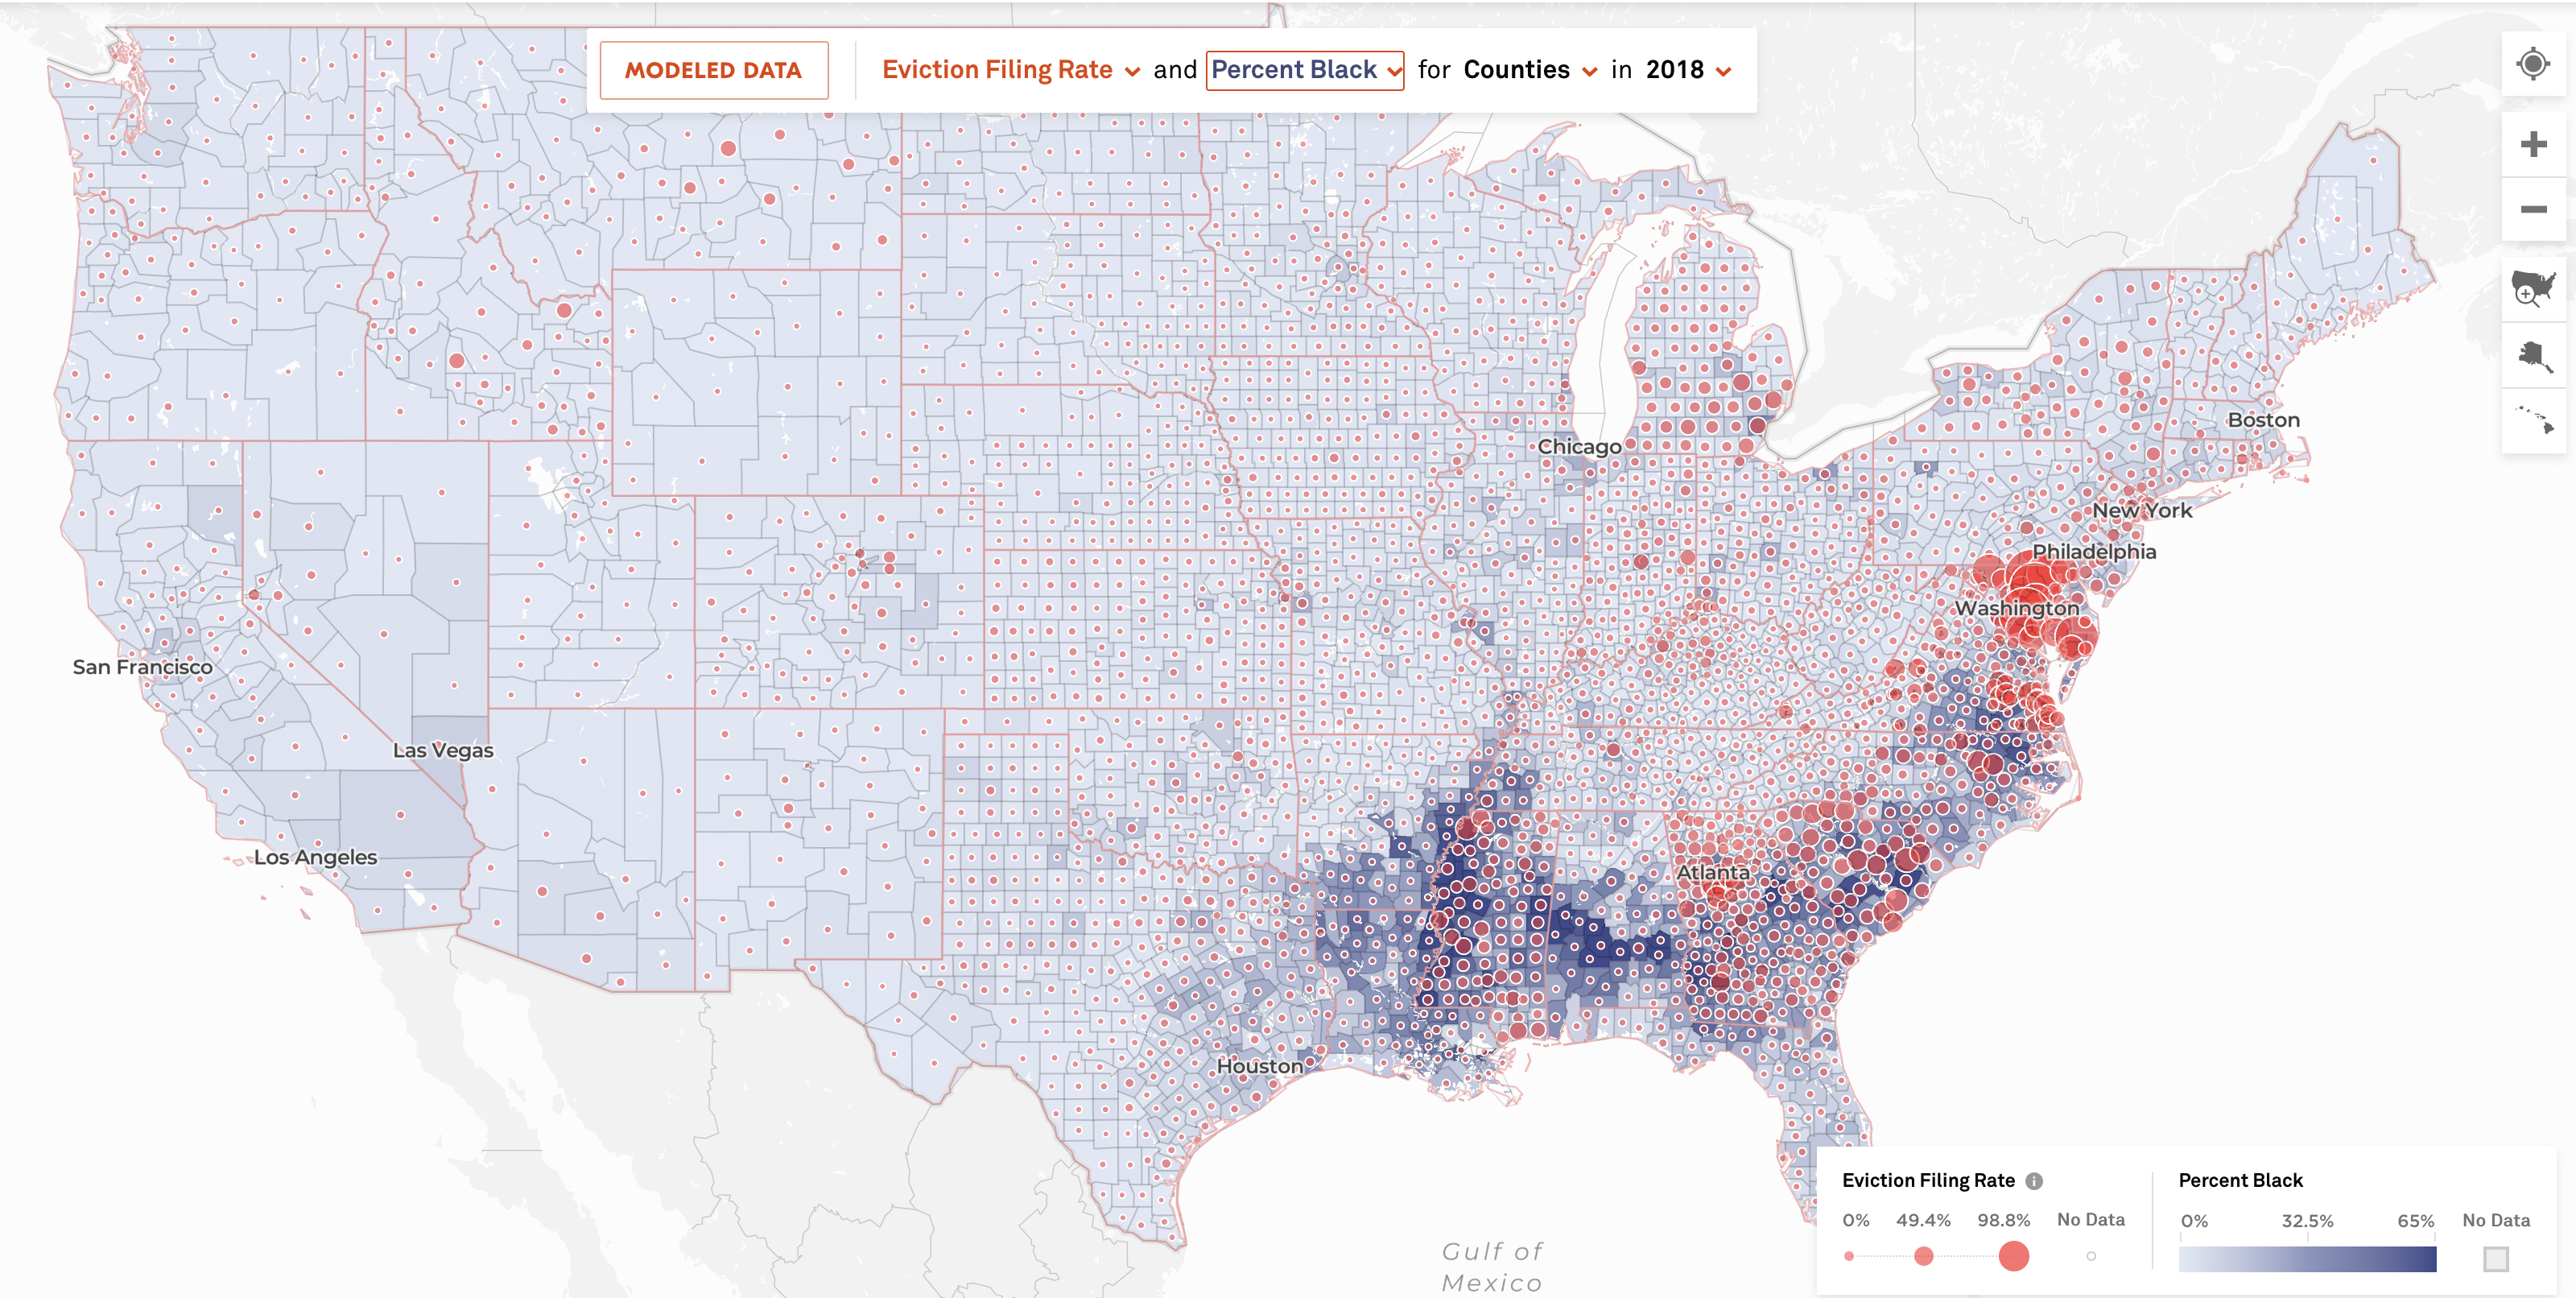
\includegraphics[width=0.65\linewidth]{figs/national-eviction-map.png}
%     \caption{Evictions in America}
%     \label{fig:natl-map}
% \end{figure}
    
% \end{frame}


% \begin{frame}{Evictions in Philadelphia: Map}
% \begin{figure}
%     \centering
%     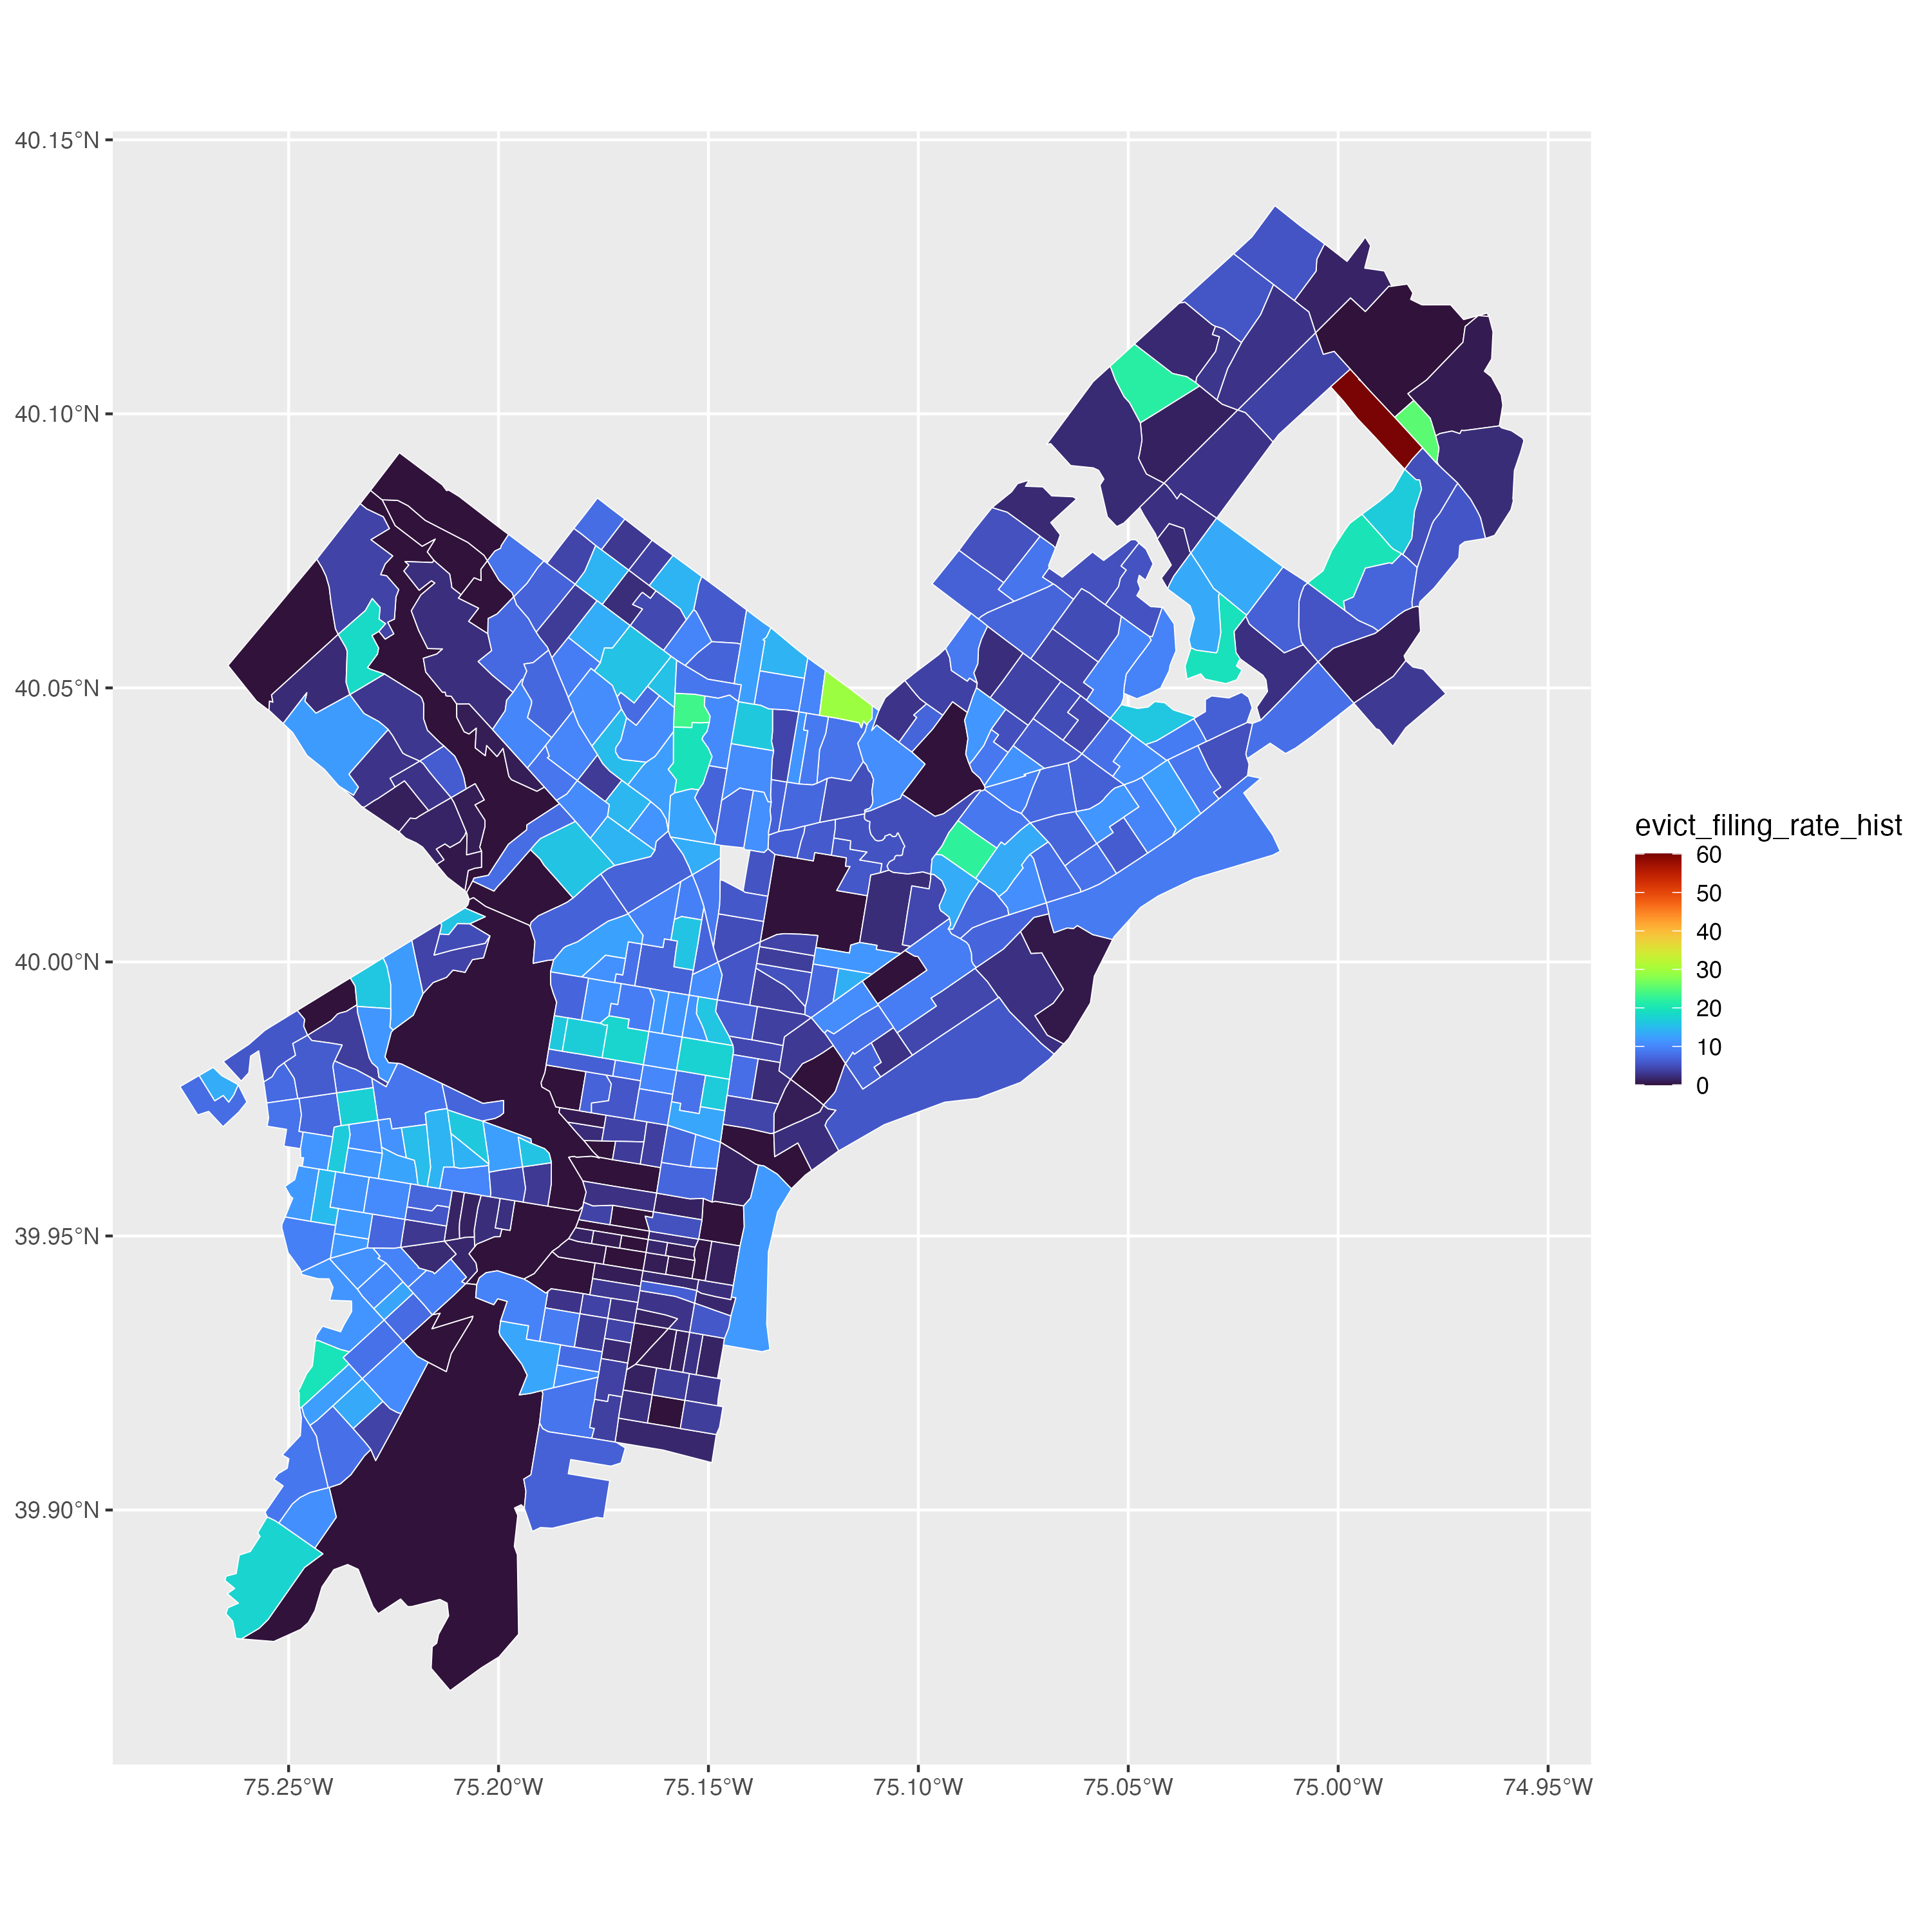
\includegraphics[width=0.6\linewidth]{figs/evict_filing_rate_hist.png}
%     \caption{Evictions in Philadelphia}
%     \label{fig:philly-map}
% \end{figure}
    
% \end{frame}

% \begin{frame}{Evictions in Philadelphia: Tracts}
% \begin{figure}
%     \centering
%     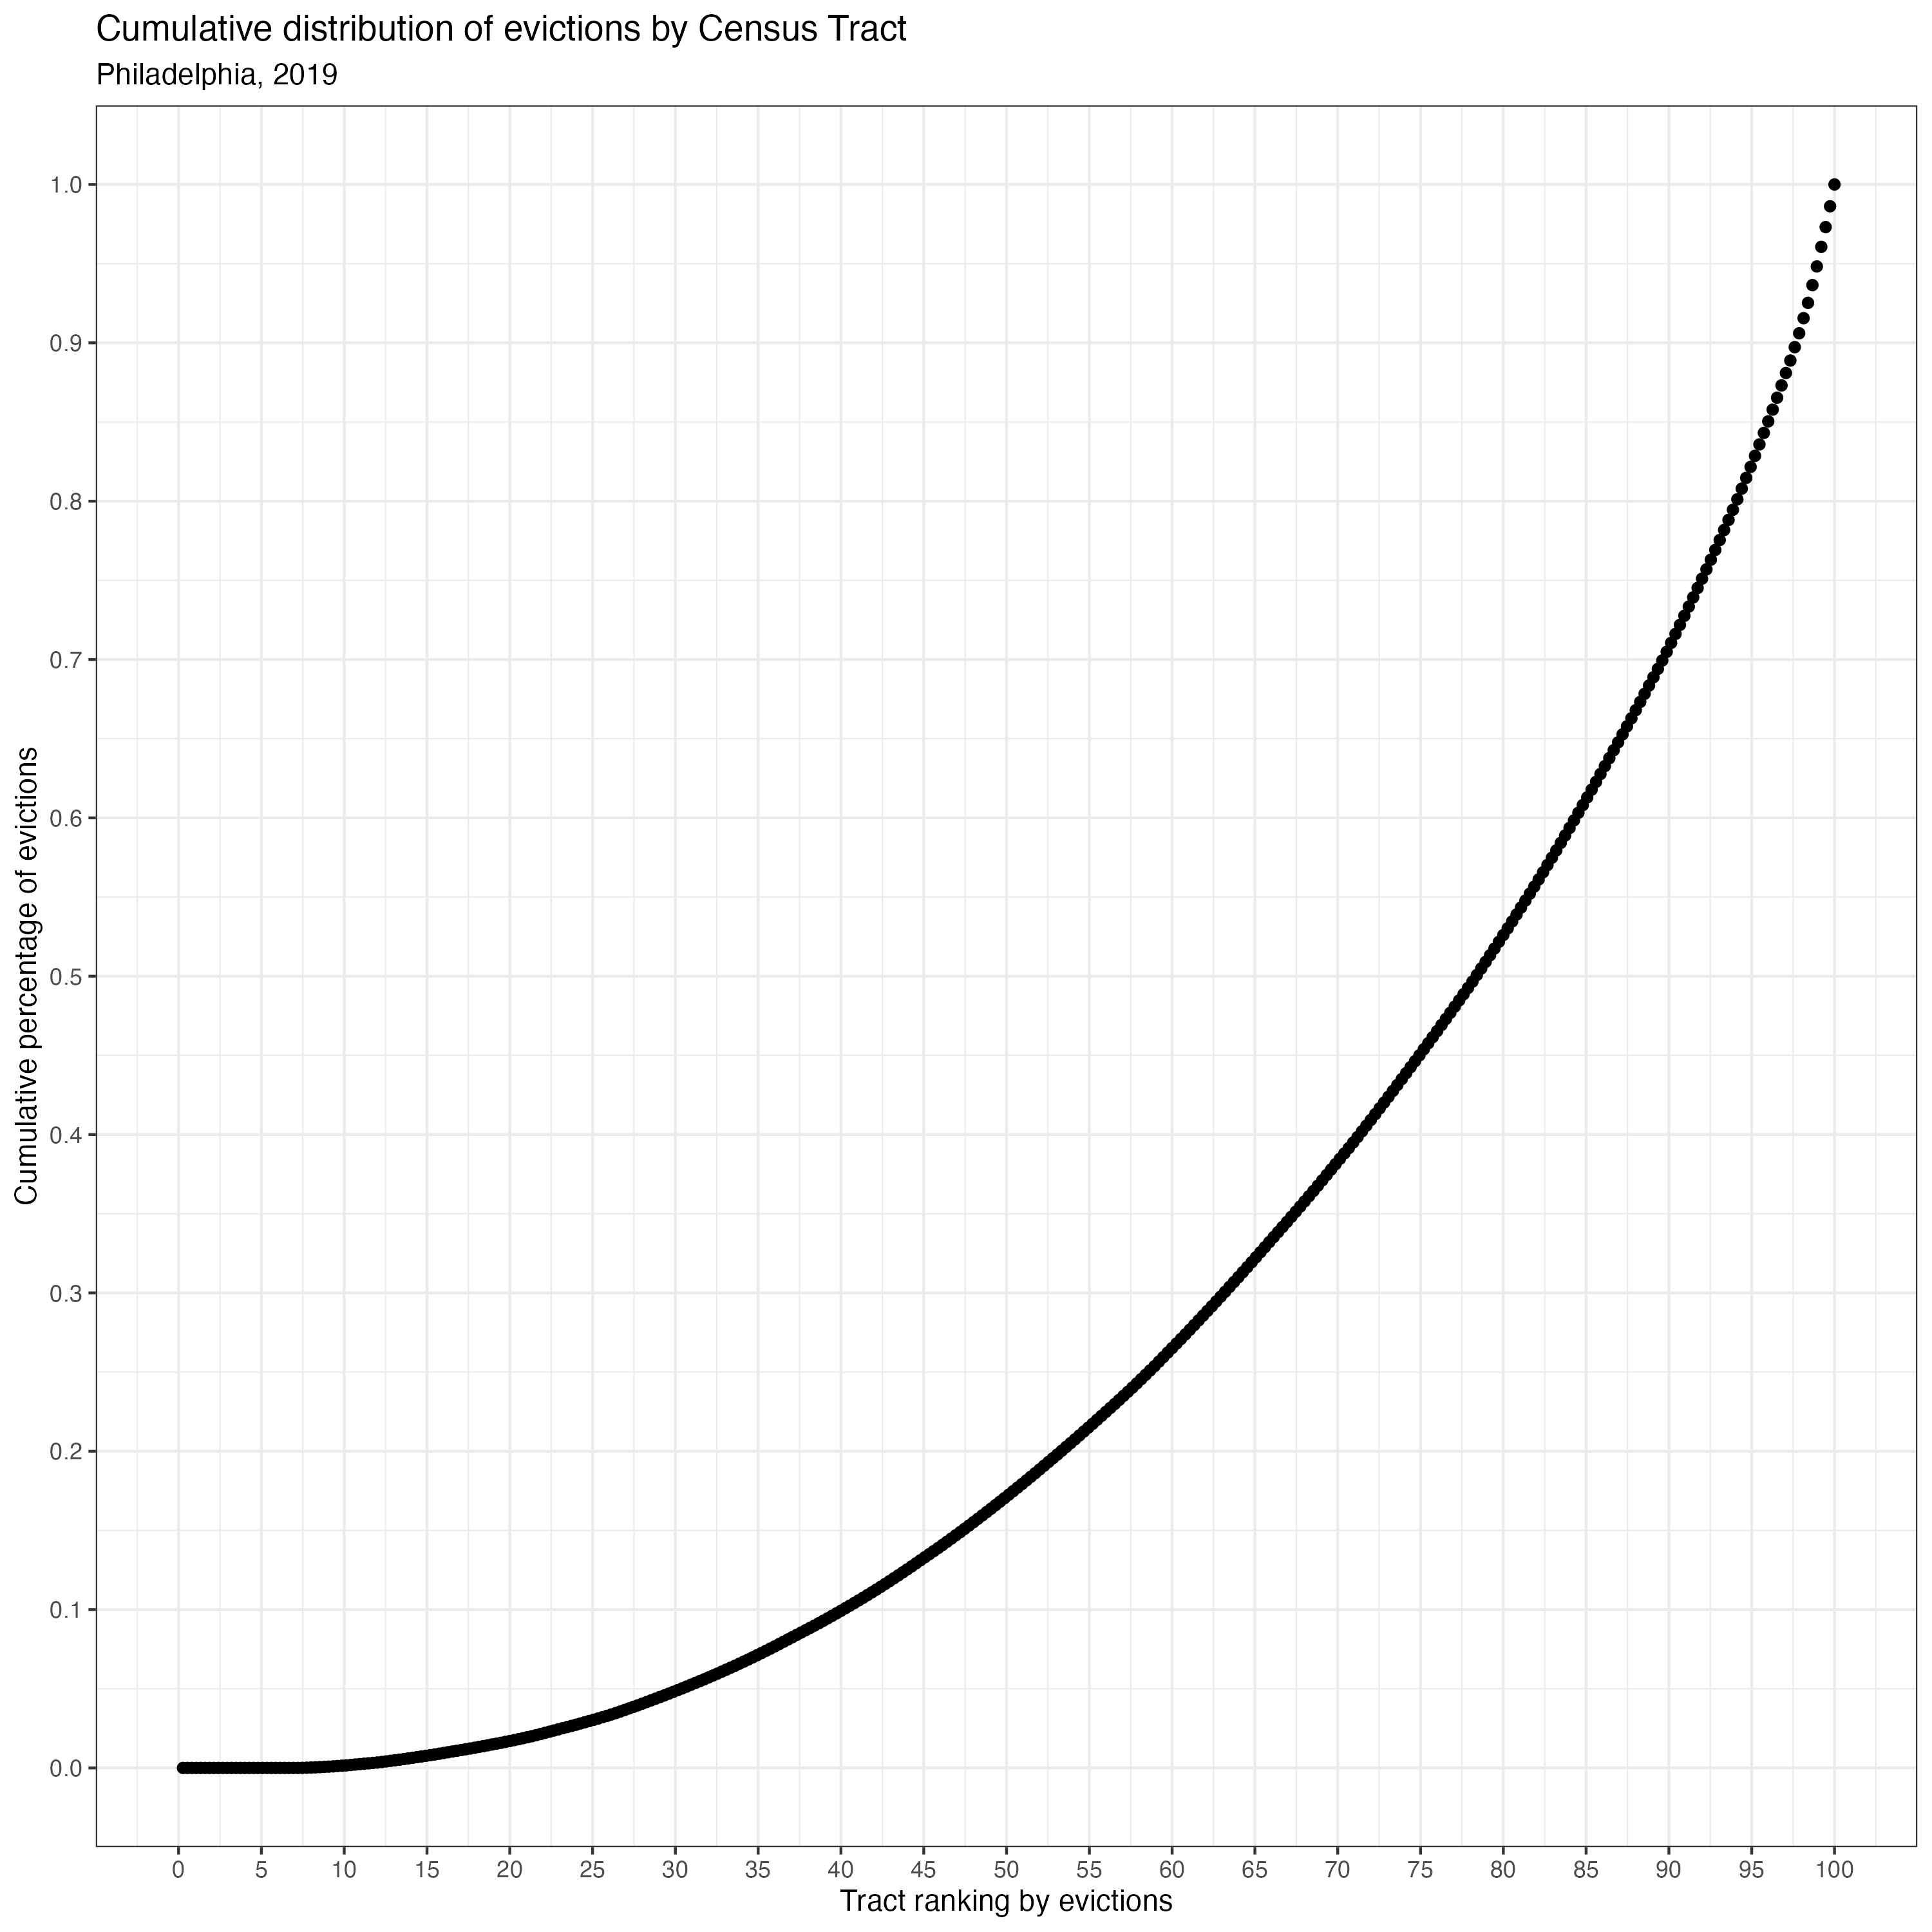
\includegraphics[width=0.6\linewidth]{figs/cumulative_evict_dist.png}
%     \caption{CDF of Evictions by Census Tract}
%     \label{fig:cum-tract}
% \end{figure}
    
% \end{frame}

% \begin{frame}{Evictions in Philadelphia: Addresses}
% \begin{figure}
%     \centering
%     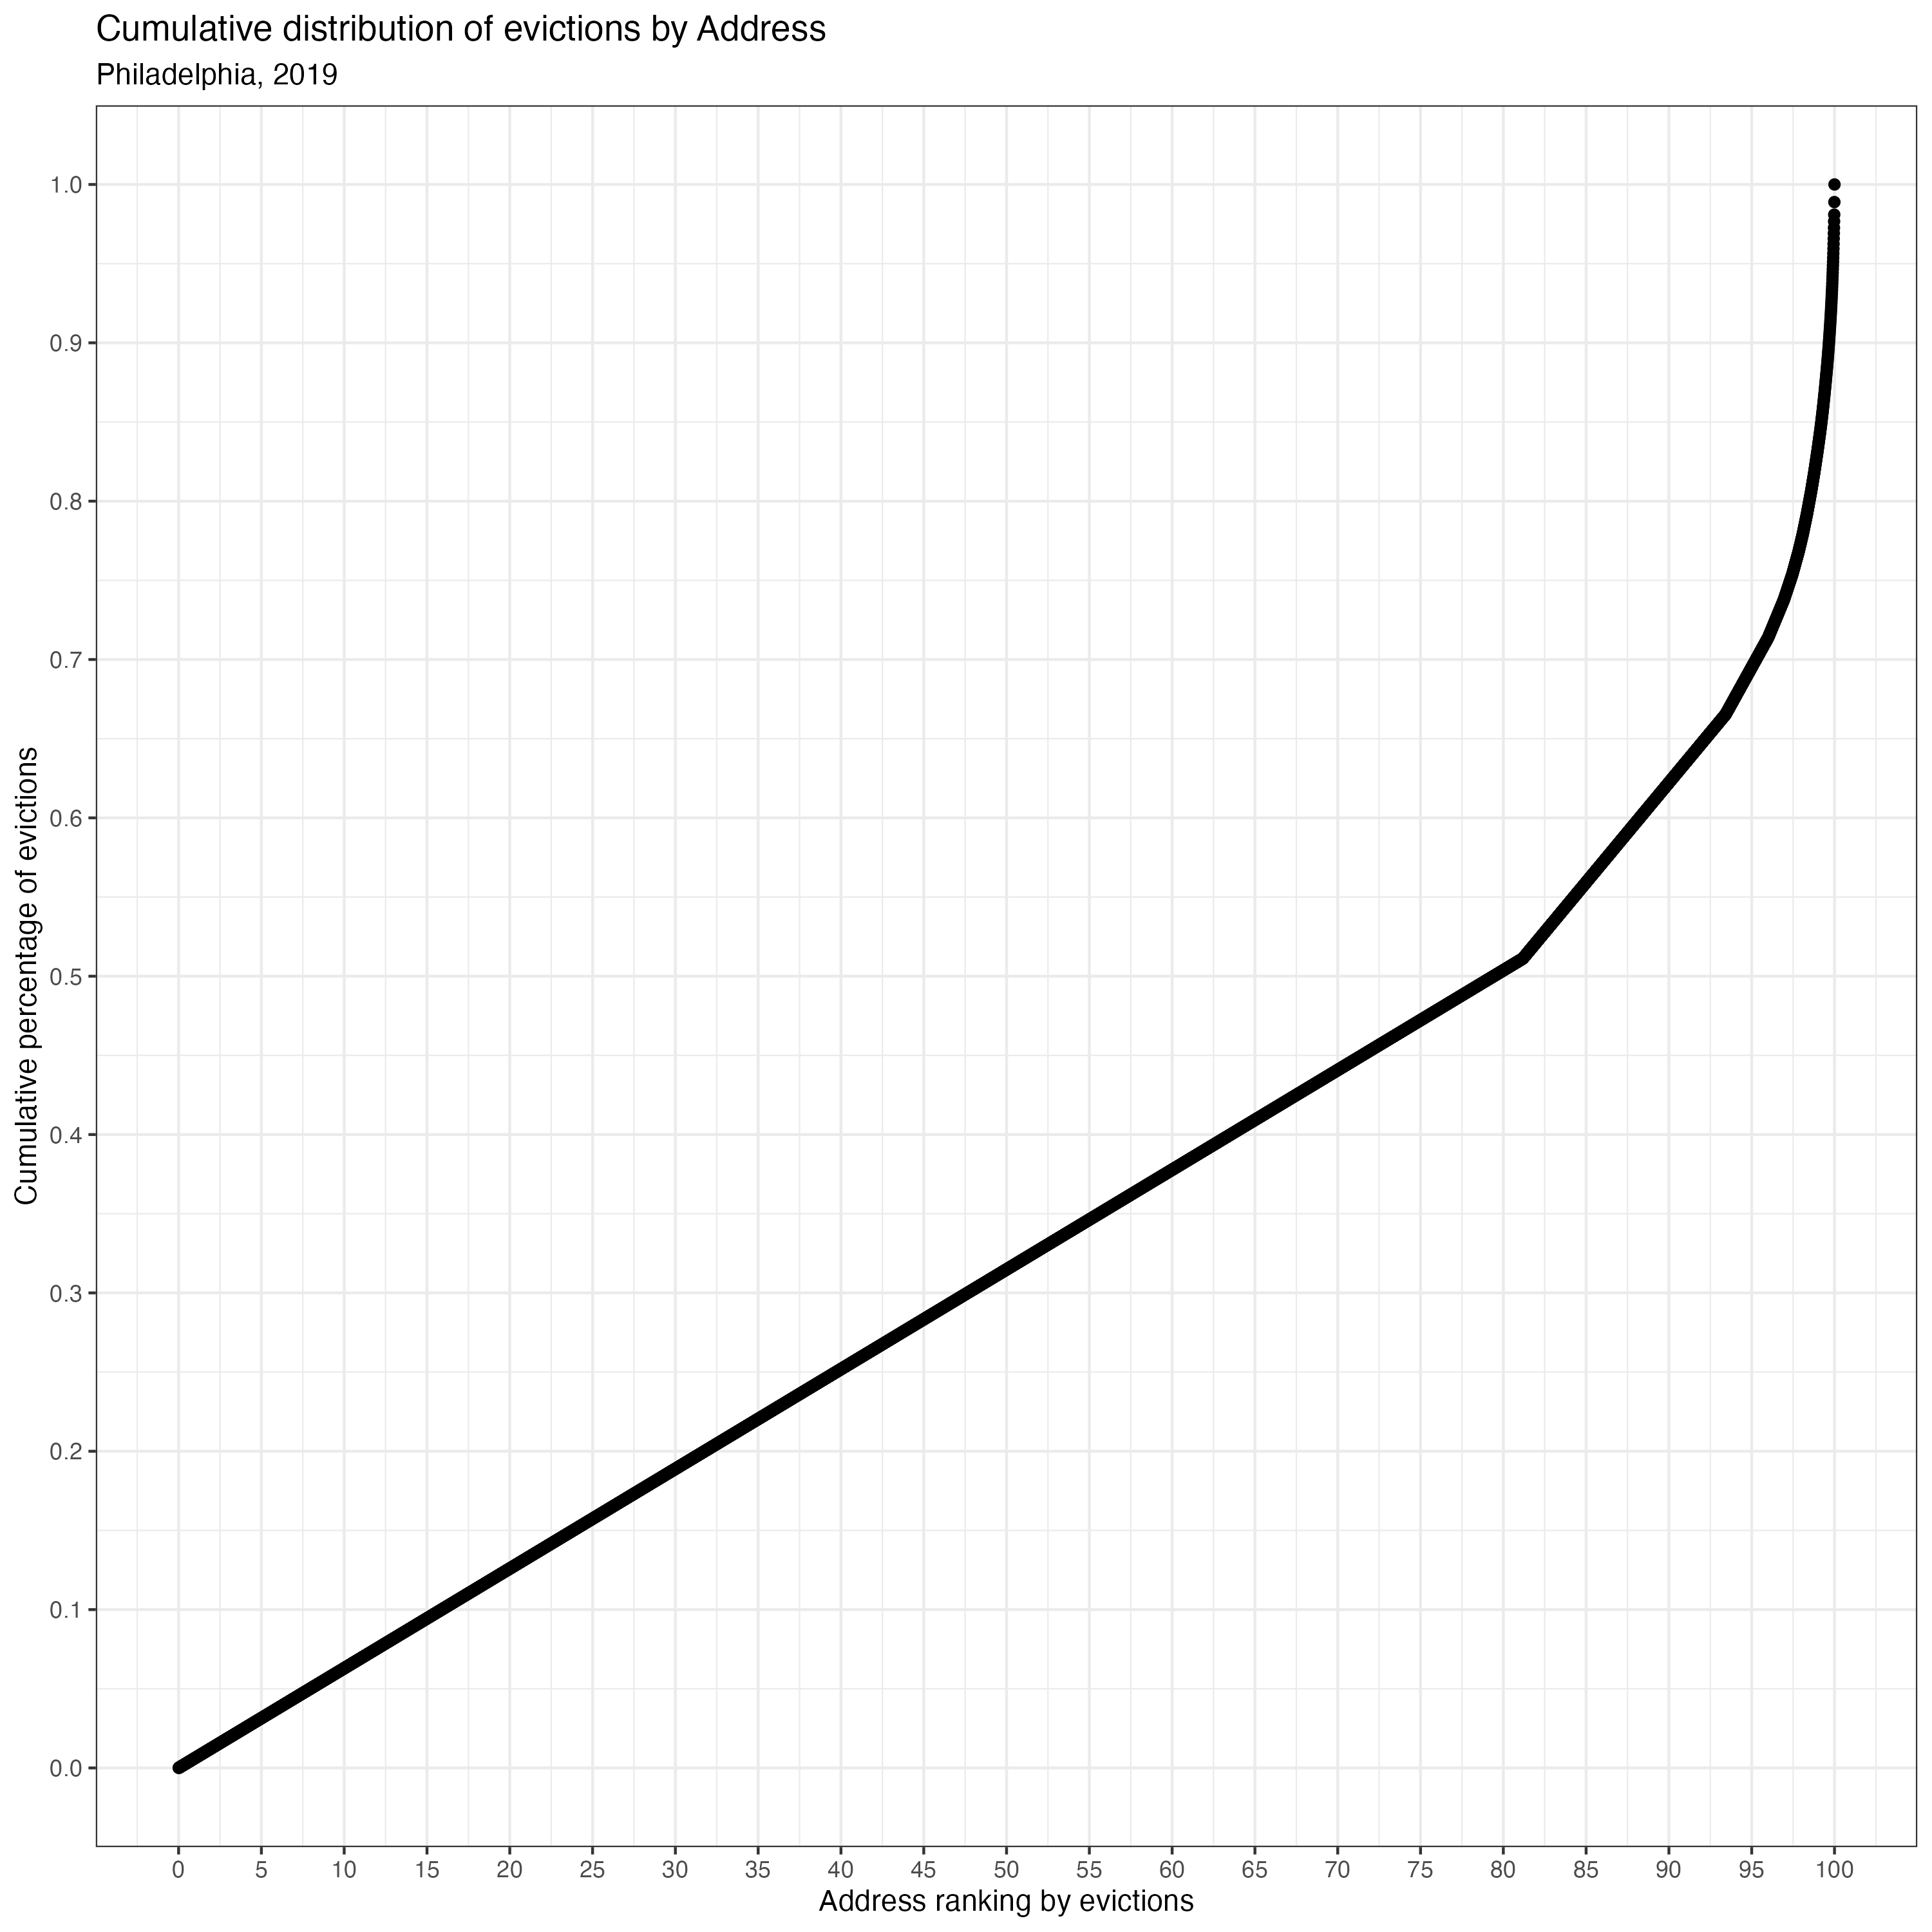
\includegraphics[width=0.6\linewidth]{figs/cumulative_evict_dist_address_hist.png}
%     \caption{CDF of Evictions by Address}
%     \label{fig:cum-address}
% \end{figure}
    
% \end{frame}

% \begin{frame}{Evictions in Philadelphia: Plaintiffs}
% \begin{figure}
%     \centering
%     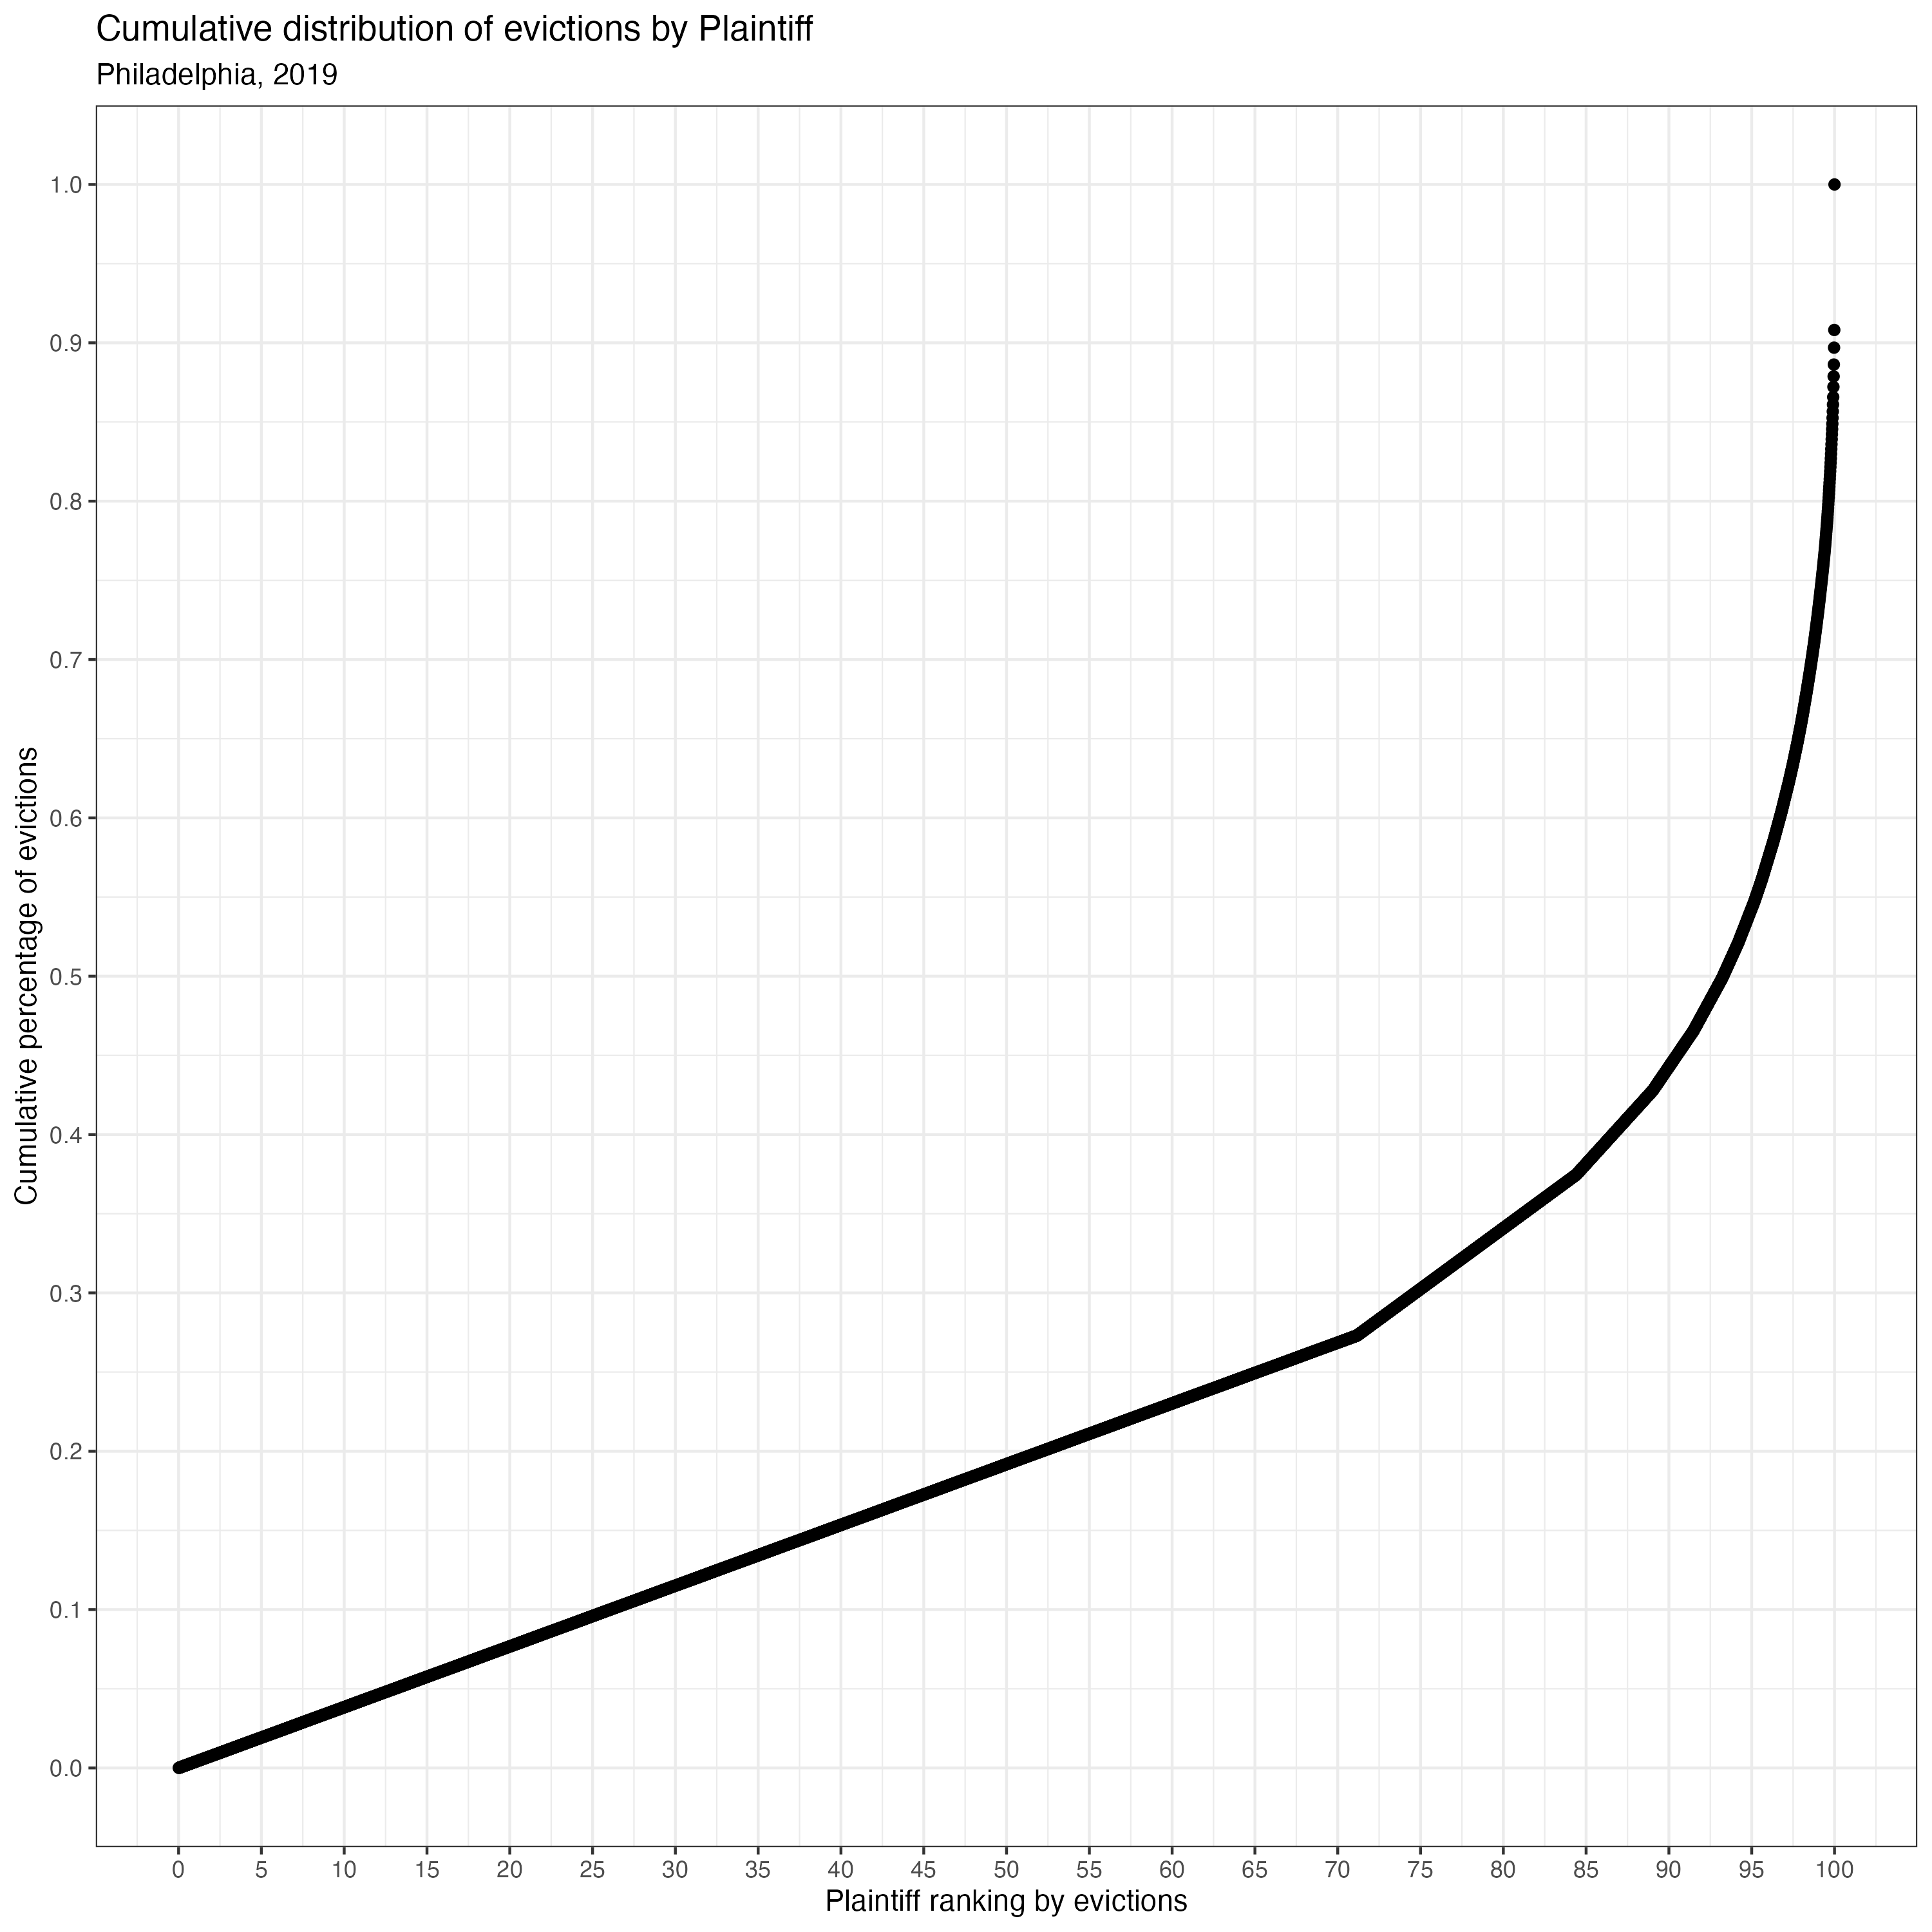
\includegraphics[width=0.6\linewidth]{figs/cumulative_evict_dist_plaintiff_hist.png}
%     \caption{CDF of Evictions by Plaintiff Name}
%     \label{fig:cdf-plaintiff}
% \end{figure}
    
% \end{frame}


\end{document}
